% The packed bed: capsules in a column, the fluid flowing through the voids
\documentclass[tikz, border=4pt]{standalone}
% Shared preamble of the PyTES model diagrams: packages, colours and styles.
% Each diagram is a standalone document that inputs this file; build them with build.py.
\usepackage{amsmath}
\usepackage{bm}
\usetikzlibrary{arrows.meta, calc, decorations.pathreplacing, patterns, positioning}

% The PyTES Thermal colour cycle (pytes.plotting.THERMAL) and tints of it
\definecolor{pytesorange}{HTML}{E8590C}
\definecolor{pytesblue}{HTML}{1F4E9C}
\definecolor{pytesteal}{HTML}{14A08A}
\definecolor{pytesamber}{HTML}{F0A930}
\definecolor{pytesplum}{HTML}{A23B72}
\definecolor{pytessky}{HTML}{88C7F0}
\definecolor{pytesink}{HTML}{36312E}

% Materials: the heat transfer fluid, the PCM, the metal (fins and tubes)
\colorlet{fluidfill}{pytessky!75}
\colorlet{pcmfill}{pytesamber!55}
\colorlet{liquidfill}{pytesorange!60}
\colorlet{metalfill}{pytesink!45}
\colorlet{compositefill}{pcmfill!85!metalfill}

\tikzset{
  >={Stealth[length=2.2mm]},
  every picture/.style={line join=round, line cap=round, font=\small},
  outline/.style={draw=pytesink, line width=0.6pt},
  fluid/.style={outline, fill=fluidfill},
  pcm/.style={outline, fill=pcmfill},
  liquid/.style={outline, fill=liquidfill},
  metal/.style={outline, fill=metalfill},
  composite/.style={outline, fill=compositefill},
  flow/.style={->, draw=pytesblue, line width=1.2pt},
  heat/.style={->, draw=pytesorange, line width=1.1pt},
  axis/.style={->, draw=pytesink, line width=0.7pt},
  dimension/.style={<->, >={Stealth[length=1.6mm]}, draw=pytesink, line width=0.5pt},
  guide/.style={draw=pytesink!60, line width=0.4pt, dashed},
  symmetry/.style={draw=pytesink, line width=0.5pt, dash dot},
  label/.style={text=pytesink, font=\small},
  note/.style={text=pytesink, font=\footnotesize, align=center},
}

\begin{document}
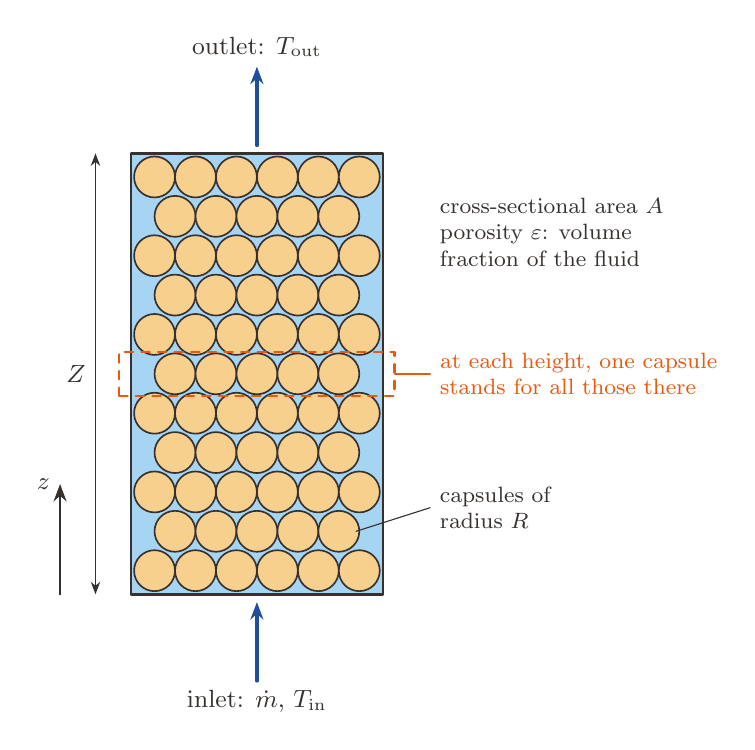
\begin{tikzpicture}
  \def\W{3.2}
  \def\Z{5.6}
  \def\rc{0.26}
  % Fluid in the voids, then the capsules in staggered rows
  \fill[fluidfill] (0, 0) rectangle (\W, \Z);
  \foreach \row in {0, ..., 10} {
    \pgfmathsetmacro{\yc}{0.3 + 0.5*\row}
    \pgfmathsetmacro{\shift}{mod(\row, 2) == 0 ? 0.3 : 0.56}
    \foreach \col in {0, ..., 5} {
      \pgfmathsetmacro{\xc}{\shift + 0.52*\col}
      \ifdim \xc pt < 3.0pt
        \draw[pcm] (\xc, \yc) circle (\rc);
      \fi
    }
  }
  \draw[outline, line width=1pt] (0, 0) rectangle (\W, \Z);
  % One height: every capsule there is the same
  \draw[pytesorange, line width=0.9pt, dashed] (-0.15, 2.52) rectangle (\W + 0.15, 3.08);
  \draw[pytesorange, line width=0.5pt] (\W + 0.15, 2.8) -- (\W + 0.6, 2.8)
    node[note, anchor=west, text=pytesorange, align=left]
    {at each height, one capsule\\stands for all those there};
  % Flow
  \draw[flow] (\W/2, -1.1) -- (\W/2, -0.1);
  \node[label, anchor=north] at (\W/2, -1.1) {inlet: $\dot m$, $T_\mathrm{in}$};
  \draw[flow] (\W/2, \Z + 0.1) -- (\W/2, \Z + 1.1);
  \node[label, anchor=south] at (\W/2, \Z + 1.1) {outlet: $T_\mathrm{out}$};
  % Coordinate and dimensions
  \draw[axis] (-0.9, 0) -- (-0.9, 1.4) node[label, left] {$z$};
  \draw[dimension] (-0.45, 0) -- (-0.45, \Z) node[label, midway, left] {$Z$};
  \node[note, anchor=west, align=left] at (\W + 0.6, 4.6)
    {cross-sectional area $A$\\porosity $\varepsilon$: volume\\fraction of the fluid};
  \node[note, anchor=west, align=left] at (\W + 0.6, 1.1)
    {capsules of\\radius $R$};
  \draw[pytesink, line width=0.4pt] (\W + 0.6, 1.1) -- (2.86, 0.8);
\end{tikzpicture}
\end{document}
